% !TEX encoding = UTF-8 Unicode

\documentclass[a4paper]{article}

\usepackage{color}
\usepackage{url}
\usepackage[T2A]{fontenc} % enable Cyrillic fonts
\usepackage[utf8]{inputenc} % make weird characters work
\usepackage{graphicx}
\usepackage{listings}
\usepackage{subfig}

\usepackage[english,serbian]{babel}

\usepackage[unicode]{hyperref}
\hypersetup{colorlinks,citecolor=green,filecolor=green,linkcolor=blue,urlcolor=blue}

%\newtheorem{primer}{Пример}[section] %ćirilični primer
\newtheorem{primer}{Primer}[section]

\begin{document}

\title{Lokalna pretraga za dninamički lokacijski problem maksimalnog pokrivanja\\ \small{Seminarski rad u okviru kursa\\Naučno izračunavanje\\ Matematički fakultet}}

\author{Rastko Đorđević, 1091/2017\\ rastko\_djordjevic@matf.bg.ac.rs}
\maketitle

\abstract{
Dinamički lokacijski problem maksimalnog pokrivanja\textit{(eng. Dynamic maximal covering location problem, DMCLP)} na velikoj količini podataka je interesantna oblast istraživanja. U ovom radu će biti opisan problem, metoda lokalne pretrage, i implementacija metode za dati problem u programskom jeziku Python.}

\tableofcontents

\newpage



\section{Postavka problema}

Postavka problema koja će biti objašnjena u nastavku je inspirisana radom\cite{main_paper}. Dobro poznati tip lokacijskih problema koje je izučavan od samog početka oblasti je lokacijski problem pokrivanja u kojem je cilj prekriti skup zahteva uz određeni cilj koji treba optimizovati. Verzija koja će biti razmatrana u ostatku rada je lokacijski problem maksimalnog pokrivanja u kojem je cilj pokriti maksimalan broj zahteva sa poznatim brojem objekata. Pored toga problem će biti još zakomplikovan uvođenjem više perioda.  U takvom problemu cilj je pronaći optimalnu lokaciju za p objekata u m različitih perioda.

\subsection{Matematička definicija}

Kako bismo predstavili DMCLP neophodno je postaviti neke pretpostavke. U daljem radu biće podrazumevano da se koristi diskretni tip problema. Takođe proizvoljni čvor se računa kao pokriven ako se objekat nalazi u dozvoljenoj udaljenosti od njega. Dodatno, skup zahtevnih čvorova je jedan skupu potencijalnih lokacija objekata. Svakom čvoru dodeljujemo vrednost u svakom periodu koja predstavlja težinu koju treba maksimizovati. Ovo možemo gledati kao potražnju datog čvora. Iako je poznat predodređen broj ukupnih objekata koje treba dodeliti ne postoji uslov o tome koliko objekata treba dodeliti u kom periodu.

U nastavku će biti dat skup parametara i promenljivih koje treba optimizovati kao i funkcija koja se maksimizuje.
\begin{description}
\item[$i, I$]  - Indeks i skup čvorova potražnje
\item[$j, J$]  - Indeks i skup čvorova potencijalnih objekata
\item[$a_{it}$] - Potražnja u čvoru $i$ u periodu t
\item[$d_{ij}$] - Najkraća distanca između čvora $i$ i objekta $j$
\item[$S$] - Maksimalna distanca koja određuje da li je čvor pokriven 
\item[$N_{i}$] - Skup čvorova takvih da postoji bar jedan objekat koji je na distanci manjoj od $S$ od njih
\item[$p$] - broj objekata koje treba postaviti
\item[$X_{jt}$] - Binarna promenjiva koja je jednaka 1 ako je objekat postavljen na čvoru $j$ u periodu $t$
\item[$Y_{it}$] - Binarna promenjiva koja je jednaka 1 ako čvor $i$ u periodu $t$ je pokriven sa bar jednim objektom koji je postavljen na distanci manjoj od S u odnosu na čvor $i$.	
\end{description}


Za ovako definisane promenljive i parametre model glasi:
$$max \sum_{t=1}^{T} \sum_{i=1}^{I} a_{it} Y_{it} $$

Tako da važe uslovi:
$$Y_{it} \leq \sum_{j \in N_{i}} Xjt, \;\;\;\;\; i \in I, t \in T  $$
$$\sum_{t=1}^{T} \sum_{j=1}^{J} X_{jt} = p $$

Funkcija cilja služi da maksimizuje ukupnu potražnju. Prvi uslov onemogućava pokrivenost čvora u čijoj S blizini se ne nalazi bar 1 objekat. Dok drugi uslov pokazuje da se p objekata raspoređuje tokom T perioda. 

\section{Lokalna pretraga}

Lokalna pretraga pripada grupi S-metaheuristika, koje se zasnivaju na poboljšavanju vrednosti jednog
rešenja. Na početku algoritma se proizvoljno ili na neki drugi način generiše početno rešenje i izračuna vrednost njegove funkcije cilja. Vrednost najboljeg rešenja se najpre inicijalizuje na vrednost početnog. Zatim se
algoritam ponavlja kroz nekoliko iteracija. U svakom koraku se razmatra rešenje u okolini trenutnog. U zavisnosti od toga kako se definiše okolina mogu se dobiti dobri ilii loši rezultati. Ukoliko je vrednost njegove funkcije cilja bolja od vrednosti funkcije cilja trenutnog rešenja, ažurira se trenutno
rešenje. Takođe se, po potrebi, ažurira i vrednost najboljeg dostignutog rešenja. Algoritam se ponavlja
dok nije ispunjen kriterijum zaustavljanja. Kriterijum zaustavljanja može biti, na primer, dostignut maksimalan broj iteracija, dostignut maksimalan broj ponavljanja najboljeg rešenja, ukupno vreme izvršavanja,
itd. Lokalna pretraga se može prikazati sledećim pseudokodom


Pseudo-kod algoritma:
\begin{verbatim}
Lokalna pretraga()
Ulaz:

Izlaz:

begin
    Generisati početno rešenje s
    Inicijalizovati vrednost najboljeg rešenja f* <= f(s)
    dok nije ispunjen izabrani kriterijum zaustavljanja do
        izabrati proizvoljno rešenje s' u okolini s koje je validno
        ako f(s') < f(s) onda
            s <= s'
        ako f(s') < f* onda
            f* <= f(s')	
end
\end{verbatim}

U datoj verziji lokalne pretrage se vrši problem minimizacije, dok je u našem problemu potrebno maksimizovati ciljnu funkciju. To ćemo rešiti tako što ćemo prihvatati ona rešenja čija je vrednost funkcije cilja veća. Osnovna mana lokalne pretrage je u tome što ne nalazi globalna rešenja, i što kada uđe u lokanlni optimum iz njega ne može da izađe. Ovo se može poboljšati korišćenjem neke naprednije tehnike koja istražuje i rešenja koja nisu trenutno najbolja u nadi da se negde dalje krije bolje rešenje.

\section{Implementacija}

Projekat je napisan korišćenjem programskog jezika Python. Implementirani su pristup grube sile i metoda lokalne pretrage nad datim problemom. Prvo će biti opisani neki od ključnih izbora kod implementacije lokalne pretrage, a dalje u nastavku je dato i kratko objašnjenje impelmentacije algoritma grube sile i poređenje njihovih brzina izvršavanja i rezultata.

\subsection{Inicijalizacija}
Inicijalizacija početnog rešenja je u potpunosti proizvoljna bez dodatnih uslova. Rešenje koje predstavlja koji od objekata je uključen u kom vremenskom periodu je predstavljeno kao jednodimenzioni niz. Potencijalni uslovi za bolje generisanje inicijalnog stanja moglo bi biti da se svakom čvoru dodeli objekat sa određenom verovatnoćom koja je srazmerna potencijalnom povećavanju potražnje njegovim dodavanjem. Problem je što iako ovo intuitivno ima smisla, ovako inicijalizovani podaci mogu slediti lošijim rešenjima.

\subsection{Izbor suseda}
Izbor okoline je takođe prostor za potencijalno poboljšanje modela. Za suseda su izabrana rešenja kod kojih se razlikuje 1 proizvoljno mesto objekta. Prvobitno je korišćena k-okolina kod kojih se lokacije k objekata razlikuju, ali algoritam znatno brže konvergira za mali broj k, tako da je u finalnom rešenju ostavljeno k=1. Takođe je razmatrana i zamena mesta ali u okviru 1 perioda i ovo je nešto što bi se moglo dodati kao potencijalni izbor suseda pored već datog rešenja.

\subsection{Algoritam grube sile}
Algoritam grube sile generiše sve moguće kombinacije rešenja i za svaku proverava kolika joj je vrednost, od kojih maksimalnu vraća kao rešenje. Budući da generiše sve kombinacije složenost algoritma je ogromna, pa čak i za male ulaze 15+ instanci izvršavanje ume da potraje, što je i očekivano.

\subsection{Rezultati}



Metoda lokalne pretrage daje iste rezultate kao i algoritam grube sile za proizvoljno generisane male test primere (broj lokacija je manji od 15). Test primeri su generisani na proizvoljan način, prvo se generiše n objekata u koordinatnom sistemu sa određenim ograničenjima potom se izračunava euklidsko rastojanje između njih i dodaju im se proizvoljne potražnje za svaki period. Lokalna pretraga se nad ovako malim test primerima pokazala kao optimalna.

Lokalna pretraga je takođe testirana i nad većim ulazima. Iz grafika \ref{fig1} se može videti da vreme izvršavanja linearno raste sa povećavanjem broja čvorova uz poprilično veliku konstantu. Za ulaze preko 500 čvorova vreme izvršavanja dostizalo je i do minut pre optimizacije izbora suseda i izračunavanja ciljne funkcije inkrementalno. Uz inkrementalno izračunavanje ciljne funkcije i las vegas pristupa izbora suseda, vreme izvršavanja se znatno poboljšalo kao što se može videti na slici \ref{fig1}. Nakon optimizacije algoritam se čak i za vrednosti od 4000 završava za manje od 20 sekunde. Ovi rezultati su dobijeni uz 15000 maksimalnih iteracija.


Takođe implementacija u nekom drugom jeziku kao što je na primer C++ bi sigurno sledilo konstantom ubrzanju programa budući da je Python poznat po sporom izvršavanju.

Nakon optimz

\begin{figure}%
	\centering
	\subfloat[brzina izvršavanja pre optimizacije]{{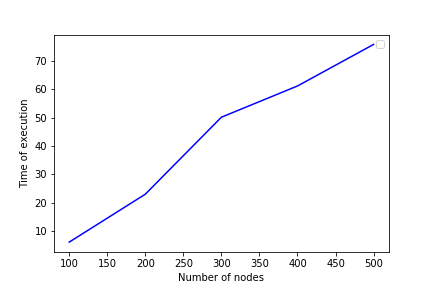
\includegraphics[width=6cm]{resources/execution_time.png} }}%
	\qquad
	\subfloat[brzina izvršavanja nakon optimizacije]{{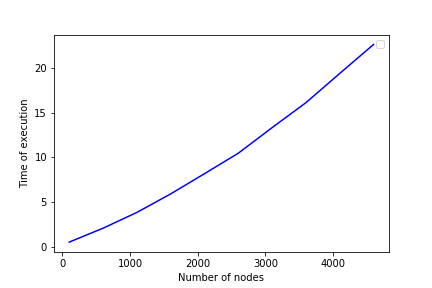
\includegraphics[width=6cm]{resources/execution_time_with_las_vegas_neighbour_gen_bigger_sample.png} }}%
	\caption{Upoređivanje brzina izvršavanja algoritama pre i posle optimizacije}%
	\label{fig1}%
\end{figure}

\section{Primene}
Lokacijski problem maksimalnog pokrivanja je klasičan model koji je našao široku primenu u raznim oblastima nauke i privrede. Dinamička verzija ovog problema je relativno nova i još istraživanja je potrebno da bi došlo do njenih primena u većem broju situacija. Ovaj model nije neuobičajen u praksi i primenljiv je u mnogim slučajevima. Na primer može se koristiti za postavku policijskih patrola \cite{police}, premeštanje ambulanti \cite{ambulance} ili realokacija mesta za prvu pomoć kod prirodnih katastrofa.

\addcontentsline{toc}{section}{Literatura}
\appendix
\bibliography{seminarski} 
\bibliographystyle{plain}

\end{document}
